%\documentclass[11pt,a4paper,titlepage,twoside]{article}
\documentclass[12pt,a4paper,twoside]{article}
%\documentclass[12pt,a4paper,twoside]{scrartcl}
\usepackage{mystyle}
\usepackage{gplot}
\usepackage{mechanik_v001}
\usepackage{foto_v001}


\usepackage[shell]{gnuplottex}
\usepackage{pgf}
\usepackage{pgfplots}
\usepackage{gnuplot-lua-tikz}
\pgfplotsset{compat=1.9}




%\author{Felix Binder}
\title{Mechanik}
\date{}



\def\dir{./Aufgaben_Mechanik/}
\newcommand{\Einbinden}[1]{\input{#1}}


\begin{document}
\maketitle

%\startkloesung

\section{Grössen und Einheiten}
\subsection{Weg}

Eine sehr wichtige Grösse in der gesamten Physik ist der Weg. 
Um die Länge eines Weges zu bestimmen muss man ihn messen.
Messen bedeutet vergleichen mit einer Einheit.
Das Formelzeichen für den Weg ist $s$. 
Die Grundeinheit (SI-Einheit, von französisch Système international d’unités) des Weges ist der Meter.
Abgekürzt wird die Einheit mit \si{m}.
Die Einheit einer physikalischen Grösse schreibt man in eckigen Klammern, also $[s]=\si{m}$.

\Einbinden{\dir/einheiten01.tex}
\Einbinden{\dir/einheiten02.tex}
\Einbinden{\dir/einheiten03.tex}
\Einbinden{\dir/einheiten04.tex}

\subsection{Zeit}
Um die Zeit $t$ zu messen, orientiert sich die Menschheit schon seit Jahrtausenden an den Gestirnen.
Winter- und Sommersonnenwenden wurden schon in der Steinzeit gefeiert.
Das Messgerät zur Zeitmessung ist die Uhr.
Die SI-Einheit der Zeit ist die Sekunde (s).
Traditionell ist die Sekunde der \num{86400}-ste Teil $(24\cdot60\cdot60)$ eines Tages.
Seit 1967 wird die Sekunde über eine atomare Anregung definiert. Daher auch der Name Atomuhr.

\Einbinden{\dir/einheiten05.tex}

\subsection{Masse}
Eine weitere häufig gebrauchte Grösse ist die Masse $m$. Ihre SI-Einheit ist das Kilogramm (kg).
Anders als bei den anderen Einheiten, hat das Kilogramm noch keine moderne, ausschliesslich auf
Naturkonstanten basierende Definition. Das Urkilogramm besteht aus einer Platin-Iridium-Legierung und wird in Paris verwahrt.


\Einbinden{\dir/einheiten06.tex}
\Einbinden{\dir/einheiten07.tex}
\Einbinden{\dir/einheiten08.tex}





\newpage

\section{Kinematik}



\Einbinden{\dir/geschwindigkeit00a.tex}
\Einbinden{\dir/geschwindigkeit00b.tex}

\Einbinden{\dir/geschwindigkeit01.tex}
\Einbinden{\dir/geschwindigkeit02.tex}
\Einbinden{\dir/geschwindigkeit03.tex}
\Einbinden{\dir/geschwindigkeit04.tex}
\newpage
\Einbinden{\dir/geschwindigkeit05.tex}

\newpage
\Einbinden{\dir/geschwindigkeit06.tex}
\Einbinden{\dir/geschwindigkeit07.tex}

\newpage

\Einbinden{\dir/beschleunigung01.tex}
\Einbinden{\dir/beschleunigung02.tex}
\Einbinden{\dir/kinematik01.tex}

\newpage
\newpage
\begin{aufgabe}
	\label{ExpWasserstrahl}
	Sie sehen ein Experiment mit einem Wasserstrahl.
	\begin{enumerate} [a)]
		\item	Schreiben Sie sich Fragen auf, die Ihnen zu diesem Experiment einfallen.
		\item	Diskutieren Sie Ihre Fragen mit Ihrem Nachbarn und versuchen Sie Antworten auf Ihre Fragen zu finden.
	\end{enumerate}

	\textbf{Tipp:} Es ist immer gut eine Skizze des Experiments anzufertigen.

\end{aufgabe}

\begin{aufgabe}
Ein Tropfen Wasser fällt aus einer Höhe von 50 Zentimeter zu Boden.
Wie lange braucht der Wassertropfen um die Erde zu erreichen?
\kloesung{\SI{0.32}{s}}
\end{aufgabe}

\begin{aufgabe}
Nehmen Sie an, Sie leben in einer Welt ohne Schwerkraft.
Was müssten Sie bei einer Wasserschlacht mit Wasserpistolen beachten?
\end{aufgabe}

\begin{aufgabe}
	Nehmen Sie an, ein Tropfen eines Wasserstrahls kommt mit einer Geschwindigkeit von \SI{2}{m/s}
	parallel zum Boden aus einem Schlauch.

	Welche Strecke $s_x$ legt der Tropfen in horizontaler Richtung zurück?
	Welche Strecke $s_y$ legt der Tropfen in Richtung des Bodens zurück?

	\begin{enumerate} [a)]
		\item	Füllen Sie die Tabelle:

	\begin{tabular}{p{4cm}|p{4cm}|p{4cm}}
			$\Delta t$ (s) & $s_x$ (m) & $s_y$ (m)\\\hline
			\num{0.1} & & \\
			\num{0.2} & & \\
			\num{0.3} & & \\
			\num{0.4} & & \\
			\num{0.5} & & \\
		\end{tabular}

	\item Zeichen Sie den Wasserstrahl mit Hilfe der berechneten Werte.
	
	\end{enumerate}
\end{aufgabe}

\newpage

\begin{aufgabe}
	In Aufgabe \ref{ExpWasserstrahl} haben Sie einen Experiment mit einem Wasserstrahl gesehen.
	Beantworten Sie zu diesem Experiment folgende Fragen:
	\begin{enumerate}[a)]
		\item	Wie lange fällt ein Wassertropfen des Wasserstrahls bis dieser den Boden erreicht.
		\item	Wie hoch ist die Geschwindigkeit des Wasserstrahls beim Austritt aus der Flasche.
	\end{enumerate}
\end{aufgabe}


\Einbinden{\dir/beschleunigung03.tex}
\Einbinden{\dir/bew3d01.tex}

\newpage
\section{Kräfte}
\Einbinden{\dir/vektoren01.tex}
\Einbinden{\dir/vektoren02.tex}
\Einbinden{\dir/vektoren03.tex}
\Einbinden{\dir/vektoren04.tex}

\begin{aufgabe}
	Sie sehen ein Experiment, bei dem zwei Ihrer Mitschüler ein Seil zwischen sich spannen.
	In die Mitte des Seils wird ein Gewicht gehängt.
	\begin{enumerate}[a)]
		\item Was beobachten Sie? Ist das Seil noch gerade oder wird das Seil durch das Gewicht geknickt?
		\item Schätzen Sie ab, mit wie viel Kraft Ihre Mitschüler an dem Seil ziehen müssen, damit es maximal einen Zentimeter durch hängt.
		\item Zeichnen Sie alle wirkenden Kräfte in einen Kräfteplan ein und bestimmen Sie die Zugkräfte im Seil
			(nehmen Sie an, das Seil ist sechs Meter lang).
			Die maximale Auslenkung soll wie bei b) sein.
	\end{enumerate}
\end{aufgabe}


%\newpage

\begin{aufgabe}
	Messen Sie in kleinen Gruppen (etwa vier Personen)
	wie ein Spielzeugauto durch das Anhängen eines Gewichtes beschleunigt wird.

	Befestigen Sie dazu einen Faden am Auto. Am anderen Ende des Fadens befestigen Sie
	Gewichte, die Sie dann über die Tischkante rutschen lassen.

	Tragen Sie die Messwerte in die Tabelle ein. 
	Berechnen Sie die Gewichtskraft, die das Auto antreibt und die Beschleunigung des Autos.
	Messen Sie auch das Gewicht des Autos.

	Tragen Sie Kraft und Beschleunigung in ein Koordinatensystem ein ($x$-Achse Beschleunigung, $y$-Achse Kraft).

\newcommand\leereZ{\phantom{x} & & & &  \\\hline}


	\begin{center}
		
		\begin{tabular}{p{0.15\textwidth}|p{0.15\textwidth}|p{0.15\textwidth}||p{0.15\textwidth}|p{0.15\textwidth}}
			\multicolumn{3}{c||}{Messwerte} & \multicolumn{2}{c}{Berechnete Grössen}\\
			$\Delta s$ (m) & $\Delta t$ (s) & $m$ (kg) & $a$ (m/s$^2$)& $F$ (N)\\\hline
			
\leereZ
\leereZ
\leereZ
\leereZ
\leereZ
\leereZ
		\end{tabular}

		\Karo{9.5}
	
	\end{center}

\end{aufgabe}


\begin{center}

\begin{tikzpicture}
  \draw [draw=none,use as bounding box] (0cm,0cm) rectangle (14cm,8cm);{
    \begin{gnuplot}[terminal=tikz,terminaloptions={size 14cm, 8cm}]
		load("../gnuplot_style")
g = 9.81
s = 0.8 #beschleunigungsstrecke daten.dat
s = 0.95 #beschleunigungsstrecke daten2.dat

f(x) = a0 + a1*x
fit f(x) "./Experimente_Mechanik/dynamik_auto/daten2.dat"  u ((2*s)/($2**2)):(($1*0.001)*g) via a0, a1 

set xlabel "Beschleunigung (m/s$^2$)"
set ylabel "Kraft (N)"


plot [0:0.6][0:] "./Experimente_Mechanik/dynamik_auto/daten2.dat" u ((2*s)/($2**2)):(($1*0.001)*g) not "F(a)" w p ls 1, f(x) not w l ls 1
    \end{gnuplot}
 };

\end{tikzpicture}
\end{center}

\begin{aufgabe}
Der Graph zeigt, wie ein Spielzeugauto durch eine Kraft $F$ beschleunigt wurde.
Die Gerade ist so zwischen die Messpunkte gelegt, dass die Summe der Abstände zu den Messpunkten möglichst klein ist.

\begin{enumerate} [a)]
	\item Beschreiben Sie den Graphen.
	\item Wie gross ist die Steigung der Geraden? Welche Einheit hat die Steigung?
	\item Wie erklären Sie sich, dass die Gerade nicht im Ursprung des Koordinatensystems beginnt?
\end{enumerate}
Die Masse der Autos beträt \SI{40.5}{g}.

\end{aufgabe}

\Einbinden{\dir/dynamik02.tex}
\Einbinden{\dir/newton02.tex}
\Einbinden{\dir/newton03.tex}

\newpage

\begin{table}
	\centering
	\begin{tabular}{ccc}
		Materialien  & Haftreibung  & Gleitreibung \\
		Holz auf Holz   &  \num{0.6}  & \num{0.4} \\
		Stahl auf Stahl &  \num{0.15} & \num{0.1}\\
		Stahl auf Eis   &  \num{0.027}& \num{0.014}\\
	\end{tabular}
	\caption{Haft- und Gleitreibungszahlen.}
	\label{tab:reibung}
\end{table}



\begin{aufgabe}
	Bestimmen Sie die Reibungszahl zwischen Tisch und Schachtel aus Aufgabe \ref{SchachtelBeschleunigungKraft}.
\end{aufgabe}

\Einbinden{\dir/reibung05.tex}
\Einbinden{\dir/reibung06.tex}
\Einbinden{\dir/reibung04.tex}
\Einbinden{\dir/reibung07.tex}

\newpage

\Einbinden{\dir/kraefte.tex}

\newpage

\begin{aufgabe}
	Wie gross war die Anfangsgeschwindigkeit eines Fahrzeugs, das längs einer waagerechten Strecke von
	\SI{200}{m} infolge der Reibung ($\mu=\num{0.02}$) zur Ruhe kommt?

	Hilfestellungen:
	\begin{enumerate} [a)]
		\item Machen Sie sich eine Skizze und tragen Sie alle Kräfte ein.
		\item Bestimmen Sie die resultierend Kraft.
		\item Setzen Sie die resultierende Kraft mit dem zweiten Newtonschen Axiom gleich.
	\end{enumerate}<++>
\end{aufgabe}


%\section{Die Dichte}

\begin{table}
	\centering
	\begin{tabular}{c r | c r | c r}
		Gold                             & 19290  & 	Sandstein     & 2400 & Ethanol  & 789\\
		Quecksilber                      & 13546  & 	Glas          &2500  & Diesel   & 830\\
		Aluminium                        &  2700  & 	Diamant       & 3510 & Olivenöl & 910\\
		Wasser (\SI{0}{\degreeCelsius})  &  1000  & 	Silber        & 10490& Meerwasser& 1025 \\
        Eis (\SI{0}{\degreeCelsius})     &   917  & 	Uran          & 19050& Milch    & 1030\\
		Holz (Kiefer)                    &   520  & 	Platin        & 21450& Helium (\SI{0}{\degreeCelsius})   & \num{0,1785}\\
		Luft                             &  1.2041& 	Blei          & 11340& Wasserstoff (\SI{0}{\degreeCelsius}) & \num{0,0899}\\
	\end{tabular}
	\caption{Dichte verschiedener Materialien in (\si{kg}/\si{m}$^3$).}
	\label{tab:dichte}
\end{table}


Die Dichte ($\rho$) ist das Verhältnis zwischen Masse (m) und Volumen (V).


\begin{cbox}
\begin{equation*}
	\rho = \frac{\text{Masse}}{\text{Volumen}} = \frac{m}{V}\text{,}\quad\text{Einheit:} [\rho]=\frac{\text{kg}}{\text{m}^3} 
\end{equation*}
\end{cbox}

Die Dichte ist eine Materialkonstante und kann zur Unterscheidung verschiedener Materialien
verwendet werden. Sie ist unabhängig von Form und Grösse des Gegenstands. 
Die Dichte von Festkörpern ist grösser als die Dichte von Gasen.
In Tabelle \ref{tab:dichte} sind die Dichten einiger Materialien angegeben.

\Einbinden{\dir/dichte01.tex}
\Einbinden{\dir/dichte02.tex}
\Einbinden{\dir/dichte03.tex}
\Einbinden{\dir/dichte04.tex}


%\section*{Weg}
%\input{./Abbildungen/weg.tex}
%\newpage
%\section{Geschwindigkeit}
Die Geschwindigkeit ist eine abgeleitete Grösse. Sie gibt an, wie viel Weg $\Delta s$ in einem Zeitintervall $\Delta t$
zurückgelegt werden.
Wenn sich weder Betrag noch Richtung der Geschwindigkeit ändern, so spricht man von einer \emph{gradlinig gleichförmig} Geschwindigkeit. 
\begin{cbox}
\begin{gather*}
	\text{Geschwindigkeit} = \frac{\text{Weg}}{\text{Zeit}}\quad\text{oder}\quad \bar{v}=\frac{\Delta s}{\Delta t}\\
		\text{Einheit}: [v] = \frac{\text{Meter}}{\text{Sekunde}}=\frac{\si{m}}{\si{s}}
\end{gather*}
\end{cbox}

Mit dem Strich über dem $\bar{v}$ wird angedeutet, dass eine durchschnittliche Geschwindigkeit
gemeint ist. Diese kann von der \emph{Momentangeschwindigkeit} abweichen, wenn das bewegte Teilchen beschleunigt wird.

\Einbinden{\dir/geschwindigkeit01.tex}
\Einbinden{\dir/geschwindigkeit02.tex}
\Einbinden{\dir/geschwindigkeit03.tex}
\Einbinden{\dir/geschwindigkeit04.tex}
\Einbinden{\dir/geschwindigkeit05.tex}


%\newpage
%\section*{Beschleunigung}
Die Beschleunigung ist eine abgeleitete Grösse. Sie gibt an, wie sich die Geschwindigkeit
mit der Zeit ändert.

Die Bewegung eines Massenpunktes heisst \emph{gradlinig gleichförmig beschleunigt}, wenn der Körper sich
mit einer konstanten Beschleunigung $a$ geradlinig bewegt.
Wird er konstant beschleunigt, ändert sich seine Geschwindigkeit linear mit der Zeit.

\begin{cbox}
\begin{gather*}
	\text{Beschleunigung} = \frac{\text{Geschwindigkeit}}{\text{Zeit}}\quad\text{oder}\quad \bar{a}=\frac{\Delta v}{\Delta t}\\
		\text{Einheit}: [a] = \frac{\text{Meter}}{\text{Sekundequadrat}}=\frac{\si{m}}{\si{s^2}}
\end{gather*}
\end{cbox}

Mit dem Strich über dem $\bar{a}$ wird angedeutet, dass eine durchschnittliche Beschleunigung 
gemeint ist.

\Einbinden{\dir/beschleunigung01.tex}
\Einbinden{\dir/beschleunigung02.tex}




\section*{Bewegungsdiagramme}
Zeitliche Bewegungsabläufe können übersichtlich in Bewegungsdiagrammen dargestellt werden.
Dabei werden die physikalischen Grössen Weg ($s$), Geschwindigkeit ($v$) und Beschleunigung ($a$) als Funktion
der Zeit dargestellt.


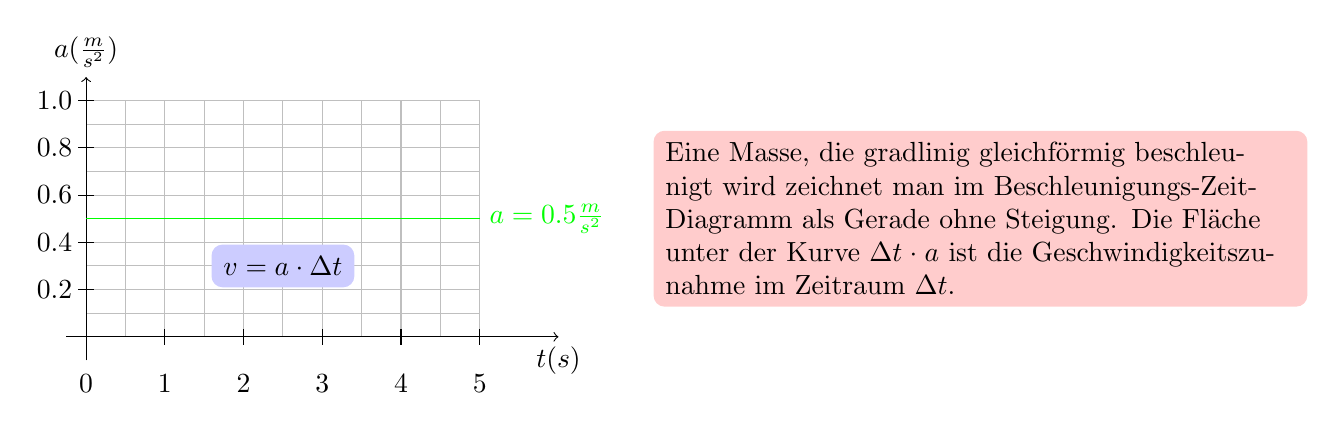
\begin{tikzpicture}[scale=1,yscale=3, info box/.style={rounded corners, inner sep=1ex}, info text/.style={info box, fill=red!20}]
\usetikzlibrary{calc,intersections,through,backgrounds}
\draw[step=0.5cm,ystep=0.1,lightgray] (0,0) grid (5.0,1.0);

%begin Koordinatensystem
%x-achse
\coordinate (C1) at (-0.25,0);
\coordinate [label=below:$t (s)$] (C2) at (6,0);
\draw  [->] (C1)--(C2);
\foreach \x in {0,1,2,3,4,5}
{
\draw (\x,-0.2) node {\x};
\draw (\x,-0.1/3)--(\x,0.1/3);
}


%y-achse
\coordinate (C3) at (0,-0.1);
\coordinate [label=above:$a (\frac{m}{s^2})$] (C4) at (0,1.1);
\draw [->] (C3)--(C4);
\foreach \y in {0.2,0.4,0.6,0.8,1.0}
{
\draw (-0.4,\y) node {\y};
\draw (-0.1,\y)--(0.1,\y);
}
%end Koordinatensystem

\draw  [color=green,domain=0:5] plot (\x,0.5) node [above,right] {$a=\SI{0.5}{\frac{m}{s^2}}$};
\draw (2.5,0.3) node [info box, fill = blue!20] {$v=a\cdot \Delta t$};

%infokasten
\draw [xshift=7.2cm] (0,0.5) node [right, text width=8cm, info text] {
Eine Masse, die  gradlinig gleichförmig beschleunigt wird zeichnet man
im Beschleunigungs-Zeit-Diagramm als Gerade ohne Steigung.
Die Fläche unter der Kurve $\Delta t\cdot a$ ist die Geschwindigkeitszunahme im Zeitraum $\Delta t$.
};



\end{tikzpicture} 


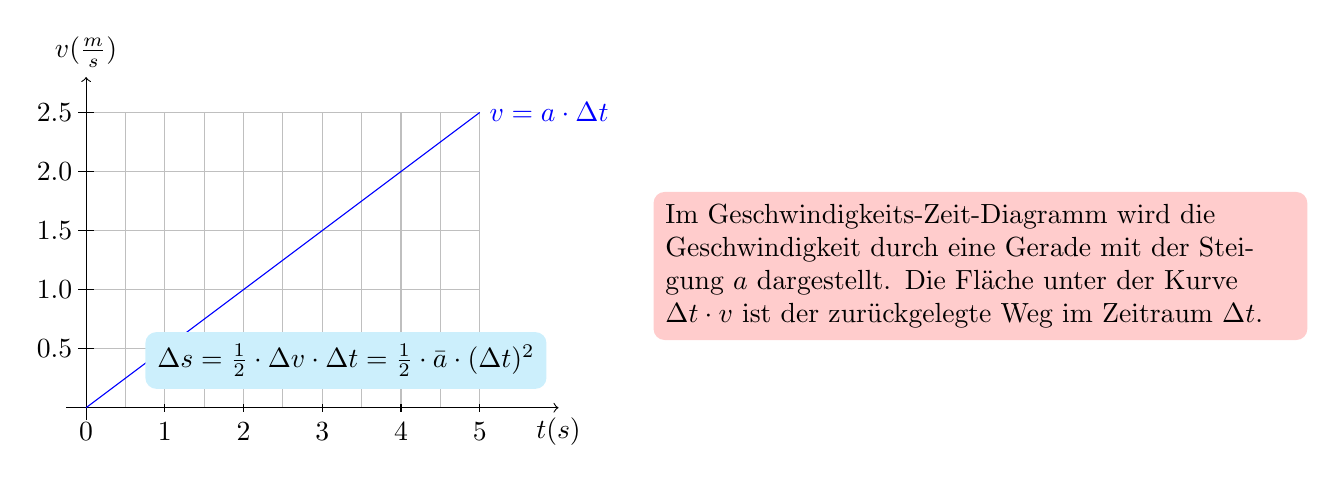
\begin{tikzpicture}[scale=1,yscale=1.5, info box/.style={rounded corners, inner sep=1ex}, info text/.style={info box, fill=red!20}]
%\usetikzlibrary{calc,intersections,through,backgrounds}
\draw[step=0.5cm,ystep=0.5,lightgray] (0,0) grid (5.0,2.5);

%begin Koordinatensystem
%x-achse
\coordinate (C1) at (-0.25,0);
\coordinate [label=below:$t (s)$] (C2) at (6,0);
\draw  [->] (C1)--(C2);
\foreach \x in {0,1,2,3,4,5}
{
\draw (\x,-0.2) node {\x};
\draw (\x,-0.1/3)--(\x,0.1/3);
}


%y-achse
\coordinate (C3) at (0,-0.1);
\coordinate [label=above:$v (\frac{m}{s})$] (C4) at (0,2.8);
\draw [->] (C3)--(C4);
\foreach \y in {0.5,1.0,1.5,2.0,2.5}
{
\draw (-0.4,\y) node {\y};
\draw (-0.1,\y)--(0.1,\y);
}
%end Koordinatensystem

\draw  [color=blue,domain=0:5] plot (\x,0.5*\x) node [above,right] {$v=a\cdot\Delta t$};
\draw (3.3,0.4) node [info box, fill =cyan!20] {$\Delta s=\frac{1}{2}\cdot \Delta v\cdot \Delta t = \frac{1}{2}\cdot\bar{a}\cdot(\Delta t)^2$};

%infokasten
\draw [xshift=7.2cm] (0,1.2) node [right, text width=8cm, info text] {
Im Geschwindigkeits-Zeit-Diagramm wird die Geschwindigkeit durch eine Gerade
mit der Steigung $a$ dargestellt. 
Die Fläche unter der Kurve $\Delta t\cdot v$ ist der zurückgelegte Weg im Zeitraum $\Delta t$.
};



\end{tikzpicture} 


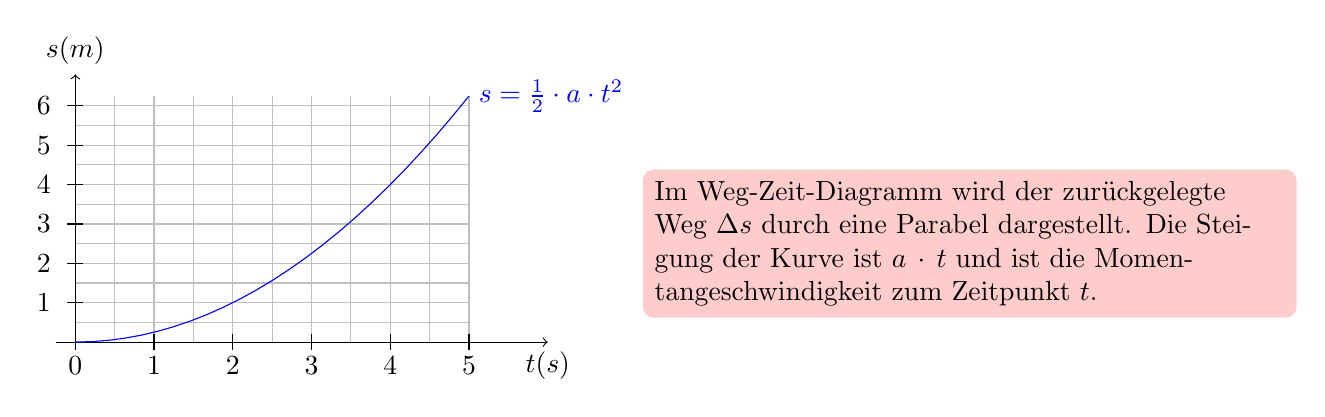
\begin{tikzpicture}[scale=1,yscale=0.5, info box/.style={rounded corners, inner sep=1ex}, info text/.style={info box, fill=red!20}]
%\usetikzlibrary{calc,intersections,through,backgrounds}
\draw[step=0.5cm,ystep=0.5,lightgray] (0,0) grid (5.0,6.25);

%begin Koordinatensystem
%x-achse
\coordinate (C1) at (-0.25,0);
\coordinate [label=below:$t (s)$] (C2) at (6,0);
\draw  [->] (C1)--(C2);
\foreach \x in {0,1,2,3,4,5}
{
\draw (\x,-0.6) node {\x};
\draw (\x,-0.1/0.5)--(\x,0.1/0.5);
}


%y-achse
\coordinate (C3) at (0,-0.1);
\coordinate [label=above:$s (m)$] (C4) at (0,6.8);
\draw [->] (C3)--(C4);
\foreach \y in {1,2,3,4,5,6}
{
\draw (-0.4,\y) node {\y};
\draw (-0.1,\y)--(0.1,\y);
}
%end Koordinatensystem

\draw  [color=blue,domain=0:5] plot (\x,0.25*\x*\x) node [above,right] {$s=\frac{1}{2}\cdot a\cdot t^2$};
%\draw (3.3,0.4) node [info box, fill =cyan!20] {$\Delta s=\frac{1}{2}\cdot \Delta v\cdot \Delta t = \frac{1}{2}\cdot\bar{a}\cdot(\Delta t)^2$};

%infokasten
\draw [xshift=7.2cm] (0,2.5) node [right, text width=8cm, info text] {
Im Weg-Zeit-Diagramm wird der zurückgelegte Weg $\Delta s$ durch eine Parabel dargestellt. 
Die Steigung der Kurve ist $a\cdot t$ und ist die Momentangeschwindigkeit zum Zeitpunkt $t$.
};



\end{tikzpicture} 




Aus den Bewegungsdiagrammen lassen sich zwei wichtige Formeln ablesen.
%\begin{cbox}
\begin{equation*}
	v=v_0+a\cdot t \qquad s=s_0 + v_0\cdot t+\frac{1}{2}\cdot a\cdot t^2
\end{equation*}
%\end{cbox}
Durch auflösen der ersten Gleichung $v=v_0+a\cdot t$ nach t und einsetzen in die zweite
bekommen wir eine Gleichung, in der die Zeit $t$ nicht vorkommt.
\begin{equation*}
	v^2=v_0^2+2\cdot a\cdot (s-s_0)
\end{equation*}

\Einbinden{\dir/beschleunigung02.tex}



%\section*{Der freie Fall}

Eine Masse fällt im Schwerefeld der Erde runter. Wie läuft der Fall der Masse ab?
Diese Frage kann mit dem Aufbau eines Experimentes beantwortet werden.
Dazu lassen wir eine Metallkugel aus einer vorher festgelegten Höhe zu Boden fallen.
Die Kugel benötigt für den Fall eine bestimmte Zeit $\Delta t$ die wir messen.
Um Fehler durch die Messung zu verringern, nehmen wir mehrere Zeitmessungen zu jeder
Höhenänderung vor und mitteln die Zeitspanne.
Dies wird für verschiedene Fallhöhen wiederholt. 
Die ermittelten Zeiten werden in einem Weg-Zeit-Diagramm eingetragen.


\begin{minipage}{0.5\textwidth}
%\begin{table}
	\centering
	\begin{tabular}{ccc}
		$\Delta s (\si{m})$ & $\Delta t (\si{ms})$ & $\overline{\Delta t} (\si{ms})$ \\\hline
0.1 & 129 131 130 & 130\\
0.2 & 195 200 201 & 199\\
0.3 & 241 248 244 & 244\\
0.4 & 278 285 276 & 280\\
	\end{tabular}
%	\caption{Messprotokoll für den freien Fall einer Metallkugel.}
%	\label{tab:freierfall1}
%\end{table}
\end{minipage}
\begin{minipage}{0.5\textwidth}
	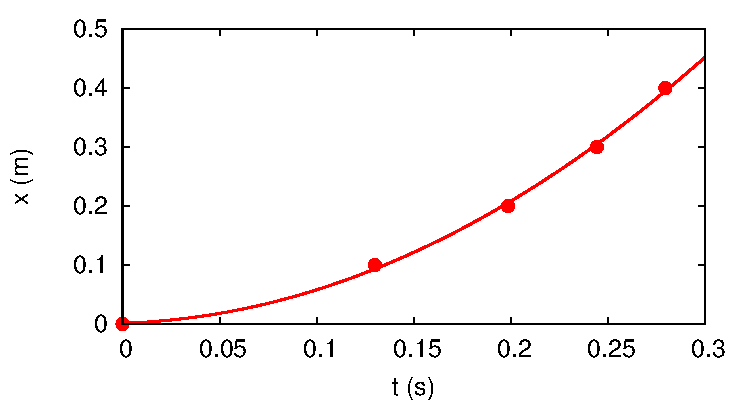
\includegraphics[width=0.95\textwidth]{./freierfall_xt.pdf}
\end{minipage}

Nun wollen wir aus dem Weg-Zeit-Diagramm ein Geschwindigkeits-Zeit-Diagramm erstellen.
Dabei gibt es einige Schwierigkeiten. Für das $v$-$t$-Diagramm wird die Momentangeschwindigkeit
benötigt. Durch die Messung kann allerdings nur eine mittlere Geschwindigkeit bestimmt werden.
Damit die mittlere Geschwindigkeit möglichst nahe an der Momentangeschwindigkeit ist, sollte eine
möglichst kleine Zeitspanne $\Delta t$ betrachtet werden.
Wir berechnen die Geschwindigkeit für die jeweils letzten \SI{10}{cm}.



\begin{minipage}{0.5\textwidth}
%\begin{table}
	\centering
	\begin{tabular}{ccc}
	$\Delta s$ &	$\Delta t (\si{s})$ & $\bar{v} (\si{m/s})$ \\\hline
%Geschwindigkeits-Zeit-Tabelle
%die letzten 10 cm
0   & 0         & 0 \\
0.1 & $\SI{130}{ms} -\SI{0}{ms}=\SI{130}{ms}$  & 0.77 \\ 
0.2 & $\SI{199}{ms} -\SI{130}{ms}=\SI{69}{ms}$  & 1.45 \\ 
0.2 & $\SI{244}{ms} -\SI{199}{ms}=\SI{45}{ms}$  & 2.22 \\ 
0.2 & $\SI{280}{ms} -\SI{244}{ms}=\SI{36}{ms}$  & 2.78 \\ 
	\end{tabular}
%	\caption{Messprotokoll für den freien Fall einer Metallkugel.}
%	\label{tab:freierfall1}
%\end{table}
\end{minipage}
\begin{minipage}{0.5\textwidth}
	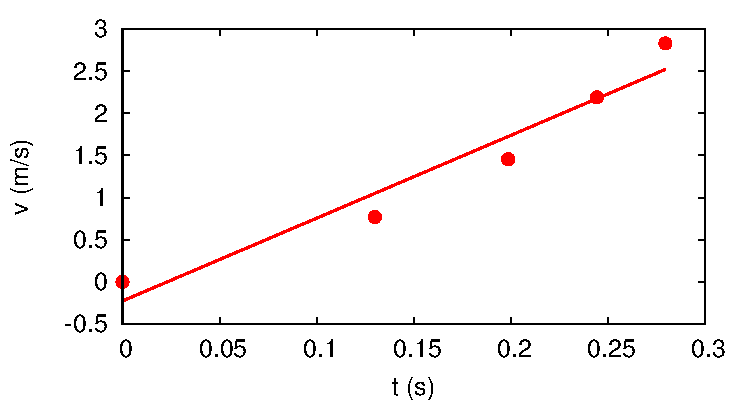
\includegraphics[width=0.95\textwidth]{./freierfall_vt.pdf}
\end{minipage}

Die berechneten Durchschnittsgeschwindigkeiten benutzen wir nun als Momentangeschwindigkeiten und tragen 
die Werte im $v$-$t$-Diagramm ein. Die Steigung der Geschwindigkeitskurve im $v$-$t$-Diagramm ist
\SI{9.92}{m/s^2}. Damit haben wir mit relativ einfachen Mitteln den Wert für die Fallbeschleunigung 
auf der Erde reproduziert und gezeigt, dass ein fallendes Objekt gleichmässig gleichförmig beschleunigt
wird, wenn es sich im Schwerefeld der Erde befindet.
Mit diesem Wissen ist es nicht mehr nötig die Momentangeschwindigkeit durch eine Durchschnittsgeschwindigkeit
zu approximieren. Stattdessen kann die Fallbeschleunigung aus dem Weg-Zeit-Diagramm bestimmt werden. 
Die Geschwindigkeit berechnet sich dann mit $v=g\cdot t$.

%\section*{Bewegung in drei Raumrichtungen}

\subsection*{Vektoren}
Physikalische Grössen wie die Geschwindigkeit $v$, die Beschleunigung $a$ oder auch der Weg $s$ sind
vektorielle Grössen. Ein Vektor hat nicht nur eine Grösse, sondern auch noch eine Richtung.
Vektoren werden daher oft als Pfeile gezeichnet. Die Länge des Pfeils ist dann der Betrag des Vektors,
die Richtung des Pfeils gibt die Richtung des Vektors an.

Ein Vektor kann mit einem geeigneten Koordinatensystem in Komponenten zerlegt werden.


Vektoren kann man graphisch addieren.

%
\section*{Addition von Kräften}

In einem Knoten laufen drei Fäden zusammen. An dem jeweils anderen Ende der Fäden ist eine Masse angehängt.
Zwei der drei Fäden werden durch Rollen umgelenkt.
Wird der Knoten aus seiner Ruhelage (Gleichgewichtslage) ausgelenkt, so pendelt sich das System wieder in diese Lage zurück.
Die Rollen lenken die Fadenkräfte um, ändern aber nicht ihren Betrag.
In der Ruhelage ist die Summe aller angreifenden Kräfte Null.

\Einbinden{\dir/vektoren01.tex}
\Einbinden{\dir/vektoren02.tex}
\Einbinden{\dir/vektoren03.tex}
\Einbinden{\dir/vektoren04.tex}


\newpage
\section*{Zerlegung von Kräften}

Vektoren lassen sich nicht nur addieren, sondern man kann sie auch in Komponenten zerlegen. Das ist im Prinzip die Umkehrung
der Vektoraddition.

\Einbinden{\dir/vektoren05.tex}
\Einbinden{\dir/vektoren06.tex}


Ist die Richtung eines Vektors vorgegeben, lässt sich der Vektor noch nicht eindeutig zerlegen. Es gibt immer
noch viele verschiedene Möglichkeiten den Vektor zu zerlegen.

\newpage


Sind die Richtungen von zwei Vektoren gegeben (in 2D), ist die Zerlegung eindeutig möglich. Allgemein gilt, dass man
für jede Raumdimension eine eindeutige Richtung benötigt.

\Einbinden{\dir/vektoren07.tex}


In der Praxis zerlegt man Vektoren oft in Kartesische Koordinaten, also in eine $x$-, eine $y$- und im Fall von drei Dimensionen in eine $z$-Koordinate.

\Einbinden{\dir/vektoren08.tex}

\newpage

\Einbinden{\dir/vektoren09.tex}

\newpage
\Einbinden{\dir/vektoren10.tex}

\Einbinden{\dir/vektoren11.tex}


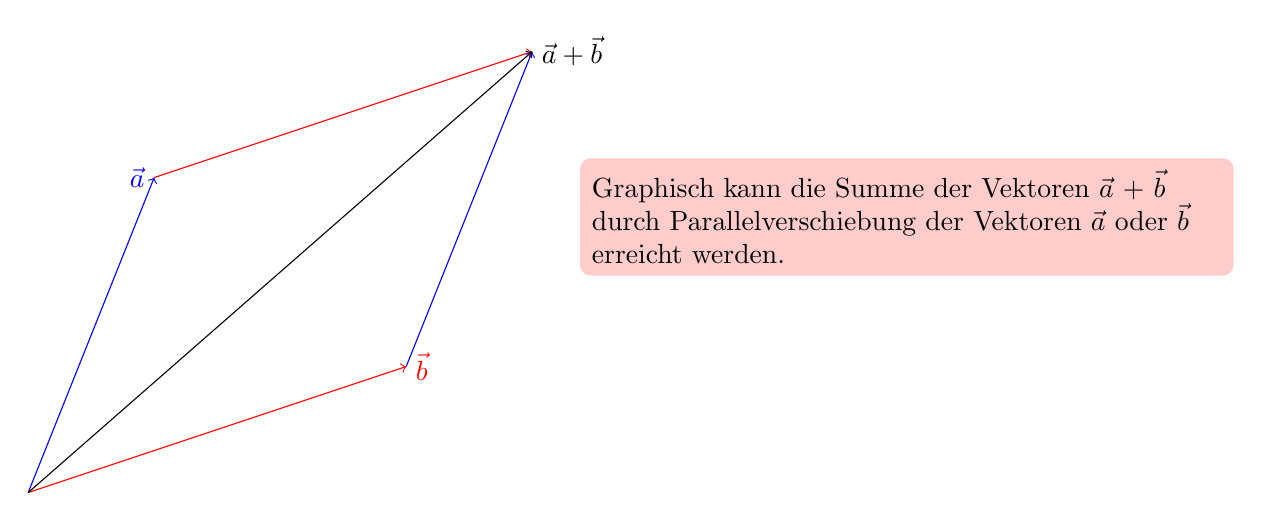
\begin{tikzpicture}[info text/.style={rounded corners, fill=red!20, inner sep=1ex}]
%\begin{tikzpicture}
%\usetikzlibrary{calc,intersections,through,backgrounds}
%\usetikzlibrary{decorations.pathmorphing}
%\draw[step=0.5cm,lightgray] (-0.5,-3.0) grid (6.5,5.0);


\draw [->, blue,scale=0.8] (0,0)--(2,5) node [left] {$\vec{a}$};
\draw[->,red,scale=0.8] (2,5)--+(6,2);

\draw[->,red,scale=0.8] (0,0)--(6,2) node [right] {$\vec{b}$};

\draw[->,blue,scale=0.8] (6,2)--+(2,5);


\draw[->,black,scale=0.8](0,0)--(8,7) node [right]{$\vec{a}+\vec{b}$};
%infokasten
\draw [xshift=7.0cm] (0,3.5) node [right, text width=8cm, info text] {
Graphisch kann die Summe der Vektoren $\vec{a}+\vec{b}$ durch Parallelverschiebung
der Vektoren $\vec{a}$ oder $\vec{b}$ erreicht werden.
};

\end{tikzpicture}

Das bedeutet, dass man eine komplizierte Bewegung, wie zum Beispiel die Bewegung eines geworfenen
Balls, oder einer Pistolenkugel für jede Raumrichtung unabhängig voneinander lösen kann.
Dies macht es erst möglich Bewegungsabläufe in mehr als einer Dimension zu berechnen.

\Einbinden{\dir/bew3d01.tex}
\Einbinden{\dir/bew3d02.tex}





%\newpage
%\printkloesung

\newpage

\section*{Die schiefe Ebene}

\begin{aufgabe}
	Sie sehen in einem Experiment einen Holzklotz auf einer Ebene liegen. 
	Die Ebene lässt sich schrägstellen. Die folgenden drei Skizzen zeigen drei
	typische Schieflagen der Ebene.
	\begin{enumerate} [a)]
		\item Machen Sie sich neben der Skizze Notizen, was mit dem Holzklotz im Experiment passiert.
		\item Zeichen Sie alle auftretenden Kräfte in die Skizzen ein (Gewichtskraft, Normalkraft, Reibungskraft).
		\item Wie ändern sich die Kräfte mit der Änderung des Winkels?
	\end{enumerate}

\subsection*{Keine Steigung der Ebene}

\Spalten{0.5}{
\begin{center}
\begin{tikzpicture}

\def\angle{0}%Winkel

\coordinate (P0) at (6,0);

\draw (0,0)--(7,0);
\draw (P0)--++(180-\angle:6);


%winkel
%\draw [->] (5,0) arc(180:180-\angle:1cm);%winkelbogen
%\draw  (P0) ++(180-0.5*\angle:0.75) node {$\alpha$};%alpha

\def\hoehe{1}
\def\breite{2}
\draw (P0) ++(180-\angle:2.25cm)--++(90-\angle:\hoehe)--++(180-\angle:\breite)--++(270-\angle:\hoehe);

%\draw [color=white] (0,-3)--(2,-3);%abstand nach unten
	\end{tikzpicture}
\end{center}
\vspace*{1.5cm}
}{0.5}{}

\subsection*{Geringe Steigung der Ebene}
\Spalten{0.5}{
\begin{center}
\begin{tikzpicture}

\def\angle{15}%Winkel

\coordinate (P0) at (6,0);

\draw (0,0)--(7,0);
\draw (P0)--++(180-\angle:6);


%winkel
\draw [->] (5,0) arc(180:180-\angle:1cm);%winkelbogen
\draw  (P0) ++(180-0.5*\angle:0.75) node {$\alpha$};%alpha

\def\hoehe{1}
\def\breite{2}
\draw (P0) ++(180-\angle:2.25cm)--++(90-\angle:\hoehe)--++(180-\angle:\breite)--++(270-\angle:\hoehe);
	\end{tikzpicture}
\end{center}
\vspace*{1.5cm}
}{0.5}{}

\subsection*{Grosse Steigung der Ebene}
\Spalten{0.5}{
\begin{center}
\begin{tikzpicture}

\def\angle{65}%Winkel

\coordinate (P0) at (6,0);

\draw (0,0)--(7,0);
\draw (P0)--++(180-\angle:6);


%winkel
\draw [->] (5,0) arc(180:180-\angle:1cm);%winkelbogen
\draw  (P0) ++(180-0.5*\angle:0.75) node {$\alpha$};%alpha

\def\hoehe{1}
\def\breite{2}
\draw (P0) ++(180-\angle:2.25cm)--++(90-\angle:\hoehe)--++(180-\angle:\breite)--++(270-\angle:\hoehe);
	\end{tikzpicture}
\end{center}
\vspace*{1.5cm}
}{0.5}{}

\end{aufgabe}

\begin{aufgabe}
	Ein Holzklotz mit dem Gewicht von \SI{300}{Gramm} liegt auf einer schiefen Ebene.
	Bei einer Steigung von \SI{35}{\degree} beginnt der Block zu rutschen.
	\begin{enumerate}[a)]
		\item Machen Sie sich eine Skizze der Situation und vervollständigen sie diese mit den auftretenden Kräften.
		\item Bestimmen Sie die Normalkraft und die Reibungskraft.
		\item Wie gross ist die Haftreibungszahl?
	\end{enumerate}
	\begin{loesung}
		\begin{enumerate} [a)]
			\item Skizze wie über der Aufgabe. 
			\item Um Normalkraft und Reibungskraft zu erhalten, muss die Gewichtskraft in eine Komponente senkrecht zur Ebene (Normalkraft)
				und eine parallel zur Ebene (Reibungskraft) zerlegt werden.
				\begin{eqnarray*}
					\RI{F}{N}=\cos\alpha\RI{F}{G}
				\end{eqnarray*}
				und
				\begin{eqnarray*}
					\RI{F}{R}=\sin\alpha\RI{F}{G}\text{.}
				\end{eqnarray*}
			\item Mit der Formel für die Reibungskraft ergibt sich die Haftreibungszahl:
				\begin{eqnarray*}
					\RI{F}{R}=\mu\cdot\RI{F}{N}\to\mu=\frac{\RI{F}{R}}{\RI{F}{N}}=\frac{\sin\alpha}{\cos\alpha}=\num{0.7}\text{.}
				\end{eqnarray*}
		\end{enumerate}
	\end{loesung}
	\kloesung{c) $\mu=\num{0.7}$}
\end{aufgabe}

\newpage

\begin{aufgabe}
	Mit Ski ($\mu=0.1$) fahren Sie einen um \SI{20}{\degree} geneigten Hang herunter.

	\begin{enumerate}[a)]
		\item Zeichnen Sie alle auftretenden Kräfte in einen Kräfteplan.
		\item Stellen Sie die resultierende Kraft auf.
		\item Welche Geschwindigkeit haben Sie nach 10 Sekunden?
	\end{enumerate}
\end{aufgabe}


\newpage
leere Seite
\newpage
\section*{Das Hebelgesetz}
Im vorigen Abschnitt haben wir uns mit Kräften beschäftigt, die in einem Punkt eines Körpers angreifen.
Hat man es mit Kräften zu tun, die parallele verlaufen, gibt es keinen gemeinsamen Angriffspunkt mehr. 
Für diesen Fall muss die bisherige Theorie erweitert werden.

\Einbinden{\dir/drehmomente01.tex}
\Einbinden{\dir/drehmomente03.tex}%Wippe
\Einbinden{\dir/drehmomente05.tex}%Mobile
\Einbinden{\dir/drehmomente02.tex}%Nussknacker
\Einbinden{\dir/drehmomente04.tex}%Zange

\Einbinden{\dir/drehmomente06.tex}
\Einbinden{\dir/drehmomente07.tex}


\begin{aufgabe}
	Welche Erfahrungen haben Sie mit dem Fahrrad fahren? Schreiben Sie einen kleinen Bericht über Ihre Erfahrungen.
	Betrachten Sie die folgenden Fragen als Hilfestellung.
	\begin{itemize}
		\item	Sie wollen eine gerade flache Strasse befahren. Welchen Gang wählen Sie dafür? Warum nehmen Sie diesen Gang?
		Welche Zahnkränze gehören zu diesem Gang? Der vordere Zahnkranz (am Pedal) hat einen grossen oder kleinen Radius?
		Der hintere Zahnkranz hat einen kleinen oder grossen Radius?

		\item Sie wollen eine steile Bergstrasse hochfahren. Welchen Gang wählen Sie nun? Welche Zahnkränze kommen nun zum Einsatz?
			Erklären Sie.

		\item Sie üben eine Kraft von \SI{100}{N} auf das Pedal aus.
			Berechnen Sie die Kraft, die am hinteren Rad auf die Strasse wirkt. Entnehmen Sie die nötigen Angaben aus der Zeichnung.
	
	\end{itemize}


	\begin{center}
	\Bildeinbinden{Velo.jpeg}{0.9}
	\end{center}

\end{aufgabe}




\section*{Der Schwerpunkt eines Körpers}
\Einbinden{\dir/schwerpunkt01.tex}%Erde Sonne
\Einbinden{\dir/schwerpunkt02.tex}%verschiedene Flaechen


\section*{Drehmomente}
Das Drehmoment ist allgemein als Kreuzprodukt zweier Vektoren definiert:

\begin{cbox}
\begin{gather*}
	\text{Drehmoment} = \text{Kreuzprodukt von Hebelarm und Kraft} \quad\text{oder}\quad \vec{M} = \vec{r}\times\vec{F}\\
	\text{Einheit}: [\vec{M}]=\text{Meter}\cdot\text{Kraft}=\si{m}\cdot\si{N}=\si{Nm}
\end{gather*}
\end{cbox}

Das bedeutet, dass die Komponente der Kraft, die senkrecht auf dem Hebelarm steht mal dem Hebelarm gerechnet werden muss.

\Spalten{0.5}{
\Beispiel Ein realer Hebelarm hat immer auch ein Eigengewicht. Seine Gewichtskraft greift am Schwerpunkt an.
Die Richtung der Gewichtskraft ist im allgemeinen nicht senkrecht zum Hebelarm. Deshalb muss man die Gewichtskraft
zerlegen, in eine Komponente senkrecht zum Hebelarm und eine Komponente parallel zum Hebelarm.
Rechnerisch ist dass hier $\sin\alpha\cdot\RI{F}{G}$. Damit ergibt sich für das Drehmoment
\begin{eqnarray*}
	M=r\cdot \RI{F}{G}\cdot \sin\alpha\text{.}
\end{eqnarray*}
}{0.5}{
\begin{center}
	\begin{tikzpicture}

\coordinate (P0) at (30:2cm);
\draw [fill] (0,0) circle (0.1); \draw (0,0) node [left] {Drehachse};
\draw [fill] (P0) circle (0.1); \draw (P0) node [left] {Schwerpunkt};
\draw (0,0) --(30:4cm) node [ above,sloped] {Hebelarm};
\draw [Kraft,->] (P0)--++(-90:3cm) node [midway, left] {\RI{F}{G}}node [shape=coordinate] (EK){};

\draw [Winkel,->] (30:1cm) arc (210:270:1cm); \draw (P0) ++(240:0.8cm) node  {$\alpha$};

\draw [dotted] (P0)--++(-60:3cm)  node [midway,right] {$\sin\alpha\cdot\RI{F}{G}$};
\draw [dotted] (EK)--++(30:2.5cm) node [shape=coordinate] (EK){};
	\end{tikzpicture}
\end{center}
}

Zum Lösen von Problemen aus der Statik kann man das Drehmoment auch benutzen. Im statischen Fall muss die Summe der
Kräfte und die Summe der Drehmomente an jedem beliebigen Punkt Null sein.
\begin{align*}
	\vec{F_1} + \vec{F_2} + \vec{F_3} + \cdots + \vec{F_n} = 0\\
	\vec{M_1} + \vec{M_2} + \vec{M_3} + \cdots + \vec{M_n} = 0
\end{align*}





\Einbinden{\dir/loesen01.tex}
\Einbinden{\dir/loesen02.tex}
\Einbinden{\dir/statik_drehmomente_bruecke01.tex}


\newpage
\section*{Kreisbewegungen}

\begin{center}
	
\begin{tikzpicture}
	
\def\Radius{4.5cm}
\def\dx{2cm}

\usetikzlibrary{calc,intersections,through,backgrounds}

\draw [dotted] (0,\Radius+1)--(0,-\Radius-1);
\draw [dotted] (\Radius+1, 0)--(-\Radius-1,0);

\draw [name path = Kreis] (0,0) circle(\Radius);
%\draw (0,0) --++(0,\Radius) node [midway, left] {$R$};

\draw [->,force] (0,\Radius) --++(\dx,0) node [midway, above] {$x$} node [shape=coordinate] (A){};
\path [name path = Radius] (A) --++ (0,-\Radius);

\path [name intersections={of=Kreis and Radius, by={G}}];

\draw [->,force] (A) -- (G) node [midway,right]{$r-y$};
\draw (0,0) -- (G) node [midway, above] {$r$};

%\draw(0,0)--(0,-\Radius)--(G)--(0,\Radius)--(0,0);

%\draw (0,0) -- (G) node [midway, above] {$r$};

%\draw (G)--++(-\Radius,0);

\draw [fill] (0,0) circle(0.1);

\end{tikzpicture}
\end{center}


An einem Kreis gilt
\begin{eqnarray*}
	r=\sqrt{x^2 + y^2}\text{.}
\end{eqnarray*}

Dies kann man auch schreiben als

\begin{eqnarray*}
	r^2 = x^2 + y^2 \qquad \text{oder} \qquad y^2=r^2-x^2\text{.}
\end{eqnarray*}

Nun soll ein Gegenstand vom Punkt $P_0$ in $x$-Richtung bewegt werden.
Der Gegenstand hat die Geschwindigkeit $v$.
Wir bewegen den Gegenstand nur ein sehr kleines Stück $\Delta x$.
\begin{eqnarray*}
	\Delta x = v\cdot \Delta t
\end{eqnarray*}

In der Zeit $\Delta t$ fällt der Gegenstand in Richtung Kreismittelpunkt (siehe Skizze)
\begin{eqnarray*}
	r-y = \frac{1}{2}\cdot a\cdot (\Delta t)^2 \to y = r - \frac{1}{2}\cdot a\cdot(\Delta t)^2\text{.}
\end{eqnarray*}

\begin{eqnarray*}
	\begin{split}
		r^2 = & x^2 + y^2\\
		    = & (v\cdot \Delta t)^2 + (r-\frac{1}{2}\cdot a\cdot (\Delta t)^2)^2\\
			= & (v\cdot \Delta t)^2 + r^2 - r\cdot a\cdot (\Delta t)^2 + \frac{1}{4}\cdot a^2 \cdot (\Delta t)^4\\
	0		= & (v\cdot \Delta t)^2 - r\cdot a\cdot (\Delta t)^2 + \frac{1}{4}\cdot a^2 \cdot (\Delta t)^4\\
	r\cdot a\cdot (\Delta t)^2		= & (v\cdot \Delta t)^2 + \frac{1}{4}\cdot a^2 \cdot (\Delta t)^4\\
	r\cdot a	= & v^2 + \frac{1}{4}\cdot a^2 \cdot (\Delta t)^2\\
	\end{split}
\end{eqnarray*}

Wir schauen nach sehr kurzer Zeit. $\Delta t$ ist also fast Null. 
Der zweite Term ist damit auch Null und es folgt

\begin{eqnarray*}
	a=\frac{v^2}{r}
\end{eqnarray*}

$a$ nennt man Zentripetalbeschleunigung.

Zu jeder Beschleunigung kann auch immer eine Kraft bestimmt werden (zur Erinnerung: $F=m\cdot a$).
Die hier vorkommende Kraft ist die Zentripetalkraft \RI{F}{Z}.


\Einbinden{\dir/kreisbewegung01.tex}
\Einbinden{\dir/kreisbewegung_kanone.tex}
\Einbinden{\dir/kreisbewegung_eimer.tex}
\Einbinden{\dir/kreisbewegung_reibung.tex}

\Einbinden{\dir/hammerwurf.tex}

\newpage


\section*{Arbeit}

\begin{aufgabe}
	Den Begriff Arbeit hört man sehr häufig.
	Gleichzeitig ist der Begriff in der Alltagswelt nicht eindeutig definiert.

Überlegen Sie sich die folgenden Fragen schriftlich.
\begin{enumerate}[a)]
	\item	Was verstehen Sie unter Arbeit?
	\item 	Wann arbeiten Sie?
\end{enumerate}

\end{aufgabe}

In der Physik ist die \emph{Arbeit} klar definiert.
\emph{Arbeit} ist das Skalarprodukt aus \emph{Kraft} und \emph{Weg}.
Die Einheit der Arbeit ist das {\bf Joule}.

Um die Arbeit zu berechnen multipliziert man also die Kraftkomponente die parallel zum Weg verläuft mit dem zurückgelegten Weg.


\begin{cbox}
\begin{gather*}
    \text{Arbeit} = \text{Kraft}\cdot{\text{Weg}}\quad\text{oder}\quad W=F\cdot s\cdot \cos \alpha\\
	\text{Einheit}: [W] = \text{Newton}\cdot\text{Meter}=\si{N}\cdot\si{m}=\frac{\si{kg}\cdot\si{m}}{\si{s^2}}\cdot \si{m}=\text{Joule}=\si{J}
\end{gather*}
\end{cbox}





So wie es unterschiedliche Kräfte gibt, unterscheidet man in der Physik auch unterschiedliche Formen von Arbeit.

\subsection*{Hubarbeit}
Um einen Körper der Masse $m$ um eine Höhe $h$ anzuheben, ist eine \emph{Hubarbeit} erforderlich.
\begin{equation*}
	W_{\text{Hub}} = F \cdot h = F_{\text{G}}\cdot h = m\cdot g\cdot h
\end{equation*}

%Im Vergleich zu seiner ursprünglichen Lage hat der Körper eine höhere potentielle Energie.

%\begin{cbox}
%\begin{equation*}
%	E_{\text{pot}} = m\cdot g\cdot h
%\end{equation*}
%\end{cbox}

\begin{aufgabe}
	Eine Masse von \SI{5}{kg} wird um \SI{3}{m} angehoben.
	Berechnen Sie die erforderliche Hubarbeit?
	\begin{loesung}
		\begin{eqnarray*}
			\RI{W}{Hub} = \RI{F}{G}\cdot s=m\cdot g\cdot s= \SI{5}{kg}\cdot\SI{9.81}{m/s^2}\SI{3}{m}=\SI{147.15}{J}
		\end{eqnarray*}
	\end{loesung}
\end{aufgabe}





\subsection*{Beschleunigungsarbeit}
Um einen Körper zu beschleunigen ist eine Kraft nötig. 
Es gilt das zweite Newtonsche Gesetz $F=m\cdot a$.
Damit ist klar, dass es auch eine Beschleunigungsarbeit gibt.
\begin{eqnarray*}
	\RI{W}{Bew}=F\cdot s=m\cdot a\cdot s=\frac{1}{2}\cdot m\cdot\left(v^2-v_0^2\right)
\end{eqnarray*}

Dabei ist $m$ die Masse, $a$ die Beschleunigung, $s$ der Weg und $v$ die Geschwindigkeit.
Im letzten Schritt haben wir für $a\cdot s$ einen Ausdruck eingesetzt, den wir durch umstellen aus der Formel
$v^2=v_0^2+2\cdot a\cdot s$ bekommen haben.

%Hat der Körper die Geschwindigkeit $v$ erreicht, so besitzt er eine \emph{kinetische Energie}.

%\begin{cbox}
%\begin{equation*}
%	\RI{E}{kin} = \frac{1}{2}\cdot m\cdot v^2
%\end{equation*}
%\end{cbox}

\begin{aufgabe}
	Ein Auto mit der Masse von \SI{1500}{kg} beschleunigt nach der roten Ampel auf \SI{50}{km/h}.
	Welche Arbeit muss der Motor dafür leisten?
	\begin{loesung}
		Zuerst sollten alle Grössen in den Grundeinheiten vorliegen.
		\begin{eqnarray*}
			v=\SI{50}{km/h}=\SI{13.89}{m/s}
		\end{eqnarray*}
		\begin{eqnarray*}
			W=\frac{1}{2}\cdot m\cdot v^2=\num{0.5}\cdot\SI{1500}{kg}\cdot(\SI{13.89}{m/s})^2=\SI{144.68}{kJ}
		\end{eqnarray*}
	\end{loesung}
\end{aufgabe}

\subsection*{Verformungsarbeit}
In diesem Abschnitt werden wir lernen, wie man die Arbeit für eine nicht konstante Kraft bestimmen kann.
Arbeit ist Kraft mal Weg. Ändert sich die Kraft über den Weg, muss man dies berücksichtigen.

\begin{figure}[h!]
\begin{center}
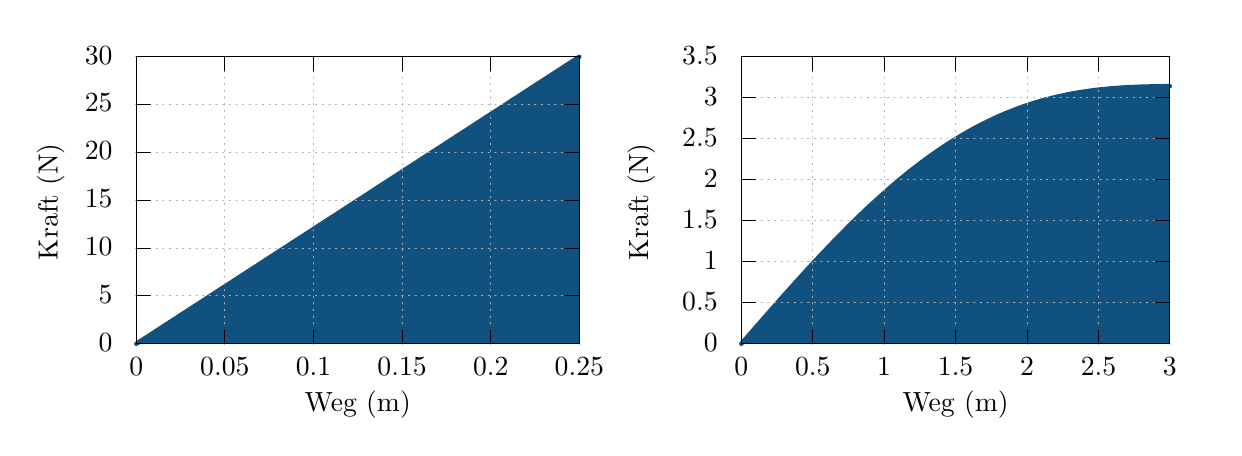
\begin{tikzpicture}[gnuplot]
%% generated with GNUPLOT 4.6p1 (Lua 5.1; terminal rev. 99, script rev. 100)
%% Mit 05 Dez 2012 16:08:51 CET
\path (0.000,0.000) rectangle (15.000,5.000);
\gpcolor{color=gp lt color border}
\gpsetlinetype{gp lt border}
\gpsetlinewidth{1.00}
\draw[gp path] (1.320,4.631)--(1.320,0.985)--(6.947,0.985)--(6.947,4.631)--cycle;
\node[gp node center,rotate=-270] at (0.246,2.808) {Kraft (N)};
\node[gp node center] at (4.133,0.215) {Weg (m)};
\gpfill{rgb color={0.063,0.318,0.502}} (1.320,0.985)--(1.320,0.985)--(1.377,1.022)--(1.434,1.059)%
    --(1.491,1.095)--(1.547,1.132)--(1.604,1.169)--(1.661,1.206)--(1.718,1.243)%
    --(1.775,1.280)--(1.832,1.316)--(1.888,1.353)--(1.945,1.390)--(2.002,1.427)%
    --(2.059,1.464)--(2.116,1.501)--(2.173,1.537)--(2.229,1.574)--(2.286,1.611)%
    --(2.343,1.648)--(2.400,1.685)--(2.457,1.722)--(2.514,1.758)--(2.570,1.795)%
    --(2.627,1.832)--(2.684,1.869)--(2.741,1.906)--(2.798,1.943)--(2.855,1.979)%
    --(2.911,2.016)--(2.968,2.053)--(3.025,2.090)--(3.082,2.127)--(3.139,2.164)%
    --(3.196,2.200)--(3.253,2.237)--(3.309,2.274)--(3.366,2.311)--(3.423,2.348)%
    --(3.480,2.384)--(3.537,2.421)--(3.594,2.458)--(3.650,2.495)--(3.707,2.532)%
    --(3.764,2.569)--(3.821,2.605)--(3.878,2.642)--(3.935,2.679)--(3.991,2.716)%
    --(4.048,2.753)--(4.105,2.790)--(4.162,2.826)--(4.219,2.863)--(4.276,2.900)%
    --(4.332,2.937)--(4.389,2.974)--(4.446,3.011)--(4.503,3.047)--(4.560,3.084)%
    --(4.617,3.121)--(4.673,3.158)--(4.730,3.195)--(4.787,3.232)--(4.844,3.268)%
    --(4.901,3.305)--(4.958,3.342)--(5.014,3.379)--(5.071,3.416)--(5.128,3.452)%
    --(5.185,3.489)--(5.242,3.526)--(5.299,3.563)--(5.356,3.600)--(5.412,3.637)%
    --(5.469,3.673)--(5.526,3.710)--(5.583,3.747)--(5.640,3.784)--(5.697,3.821)%
    --(5.753,3.858)--(5.810,3.894)--(5.867,3.931)--(5.924,3.968)--(5.981,4.005)%
    --(6.038,4.042)--(6.094,4.079)--(6.151,4.115)--(6.208,4.152)--(6.265,4.189)%
    --(6.322,4.226)--(6.379,4.263)--(6.435,4.300)--(6.492,4.336)--(6.549,4.373)%
    --(6.606,4.410)--(6.663,4.447)--(6.720,4.484)--(6.776,4.521)--(6.833,4.557)%
    --(6.890,4.594)--(6.947,4.631)--(6.947,0.985)--cycle;
\gpcolor{rgb color={0.063,0.318,0.502}}
\gpsetlinetype{gp lt plot 0}
\gpsetlinewidth{4.00}
\draw[gp path] (1.320,0.985)--(1.377,1.022)--(1.434,1.059)--(1.491,1.095)--(1.547,1.132)%
  --(1.604,1.169)--(1.661,1.206)--(1.718,1.243)--(1.775,1.280)--(1.832,1.316)--(1.888,1.353)%
  --(1.945,1.390)--(2.002,1.427)--(2.059,1.464)--(2.116,1.501)--(2.173,1.537)--(2.229,1.574)%
  --(2.286,1.611)--(2.343,1.648)--(2.400,1.685)--(2.457,1.722)--(2.514,1.758)--(2.570,1.795)%
  --(2.627,1.832)--(2.684,1.869)--(2.741,1.906)--(2.798,1.943)--(2.855,1.979)--(2.911,2.016)%
  --(2.968,2.053)--(3.025,2.090)--(3.082,2.127)--(3.139,2.164)--(3.196,2.200)--(3.253,2.237)%
  --(3.309,2.274)--(3.366,2.311)--(3.423,2.348)--(3.480,2.384)--(3.537,2.421)--(3.594,2.458)%
  --(3.650,2.495)--(3.707,2.532)--(3.764,2.569)--(3.821,2.605)--(3.878,2.642)--(3.935,2.679)%
  --(3.991,2.716)--(4.048,2.753)--(4.105,2.790)--(4.162,2.826)--(4.219,2.863)--(4.276,2.900)%
  --(4.332,2.937)--(4.389,2.974)--(4.446,3.011)--(4.503,3.047)--(4.560,3.084)--(4.617,3.121)%
  --(4.673,3.158)--(4.730,3.195)--(4.787,3.232)--(4.844,3.268)--(4.901,3.305)--(4.958,3.342)%
  --(5.014,3.379)--(5.071,3.416)--(5.128,3.452)--(5.185,3.489)--(5.242,3.526)--(5.299,3.563)%
  --(5.356,3.600)--(5.412,3.637)--(5.469,3.673)--(5.526,3.710)--(5.583,3.747)--(5.640,3.784)%
  --(5.697,3.821)--(5.753,3.858)--(5.810,3.894)--(5.867,3.931)--(5.924,3.968)--(5.981,4.005)%
  --(6.038,4.042)--(6.094,4.079)--(6.151,4.115)--(6.208,4.152)--(6.265,4.189)--(6.322,4.226)%
  --(6.379,4.263)--(6.435,4.300)--(6.492,4.336)--(6.549,4.373)--(6.606,4.410)--(6.663,4.447)%
  --(6.720,4.484)--(6.776,4.521)--(6.833,4.557)--(6.890,4.594)--(6.947,4.631);
\gpcolor{color=gp lt color axes}
\gpsetlinetype{gp lt axes}
\gpsetlinewidth{1.00}
\draw[gp path] (1.320,0.985)--(6.947,0.985);
\gpcolor{color=gp lt color border}
\gpsetlinetype{gp lt border}
\draw[gp path] (1.320,0.985)--(1.500,0.985);
\draw[gp path] (6.947,0.985)--(6.767,0.985);
\node[gp node right] at (1.136,0.985) { 0};
\gpcolor{color=gp lt color axes}
\gpsetlinetype{gp lt axes}
\draw[gp path] (1.320,1.593)--(6.947,1.593);
\gpcolor{color=gp lt color border}
\gpsetlinetype{gp lt border}
\draw[gp path] (1.320,1.593)--(1.500,1.593);
\draw[gp path] (6.947,1.593)--(6.767,1.593);
\node[gp node right] at (1.136,1.593) { 5};
\gpcolor{color=gp lt color axes}
\gpsetlinetype{gp lt axes}
\draw[gp path] (1.320,2.200)--(6.947,2.200);
\gpcolor{color=gp lt color border}
\gpsetlinetype{gp lt border}
\draw[gp path] (1.320,2.200)--(1.500,2.200);
\draw[gp path] (6.947,2.200)--(6.767,2.200);
\node[gp node right] at (1.136,2.200) { 10};
\gpcolor{color=gp lt color axes}
\gpsetlinetype{gp lt axes}
\draw[gp path] (1.320,2.808)--(6.947,2.808);
\gpcolor{color=gp lt color border}
\gpsetlinetype{gp lt border}
\draw[gp path] (1.320,2.808)--(1.500,2.808);
\draw[gp path] (6.947,2.808)--(6.767,2.808);
\node[gp node right] at (1.136,2.808) { 15};
\gpcolor{color=gp lt color axes}
\gpsetlinetype{gp lt axes}
\draw[gp path] (1.320,3.416)--(6.947,3.416);
\gpcolor{color=gp lt color border}
\gpsetlinetype{gp lt border}
\draw[gp path] (1.320,3.416)--(1.500,3.416);
\draw[gp path] (6.947,3.416)--(6.767,3.416);
\node[gp node right] at (1.136,3.416) { 20};
\gpcolor{color=gp lt color axes}
\gpsetlinetype{gp lt axes}
\draw[gp path] (1.320,4.023)--(6.947,4.023);
\gpcolor{color=gp lt color border}
\gpsetlinetype{gp lt border}
\draw[gp path] (1.320,4.023)--(1.500,4.023);
\draw[gp path] (6.947,4.023)--(6.767,4.023);
\node[gp node right] at (1.136,4.023) { 25};
\gpcolor{color=gp lt color axes}
\gpsetlinetype{gp lt axes}
\draw[gp path] (1.320,4.631)--(6.947,4.631);
\gpcolor{color=gp lt color border}
\gpsetlinetype{gp lt border}
\draw[gp path] (1.320,4.631)--(1.500,4.631);
\draw[gp path] (6.947,4.631)--(6.767,4.631);
\node[gp node right] at (1.136,4.631) { 30};
\gpcolor{color=gp lt color axes}
\gpsetlinetype{gp lt axes}
\draw[gp path] (1.320,0.985)--(1.320,4.631);
\gpcolor{color=gp lt color border}
\gpsetlinetype{gp lt border}
\draw[gp path] (1.320,0.985)--(1.320,1.165);
\draw[gp path] (1.320,4.631)--(1.320,4.451);
\node[gp node center] at (1.320,0.677) { 0};
\gpcolor{color=gp lt color axes}
\gpsetlinetype{gp lt axes}
\draw[gp path] (2.445,0.985)--(2.445,4.631);
\gpcolor{color=gp lt color border}
\gpsetlinetype{gp lt border}
\draw[gp path] (2.445,0.985)--(2.445,1.165);
\draw[gp path] (2.445,4.631)--(2.445,4.451);
\node[gp node center] at (2.445,0.677) { 0.05};
\gpcolor{color=gp lt color axes}
\gpsetlinetype{gp lt axes}
\draw[gp path] (3.571,0.985)--(3.571,4.631);
\gpcolor{color=gp lt color border}
\gpsetlinetype{gp lt border}
\draw[gp path] (3.571,0.985)--(3.571,1.165);
\draw[gp path] (3.571,4.631)--(3.571,4.451);
\node[gp node center] at (3.571,0.677) { 0.1};
\gpcolor{color=gp lt color axes}
\gpsetlinetype{gp lt axes}
\draw[gp path] (4.696,0.985)--(4.696,4.631);
\gpcolor{color=gp lt color border}
\gpsetlinetype{gp lt border}
\draw[gp path] (4.696,0.985)--(4.696,1.165);
\draw[gp path] (4.696,4.631)--(4.696,4.451);
\node[gp node center] at (4.696,0.677) { 0.15};
\gpcolor{color=gp lt color axes}
\gpsetlinetype{gp lt axes}
\draw[gp path] (5.822,0.985)--(5.822,4.451)--(5.822,4.631);
\gpcolor{color=gp lt color border}
\gpsetlinetype{gp lt border}
\draw[gp path] (5.822,0.985)--(5.822,1.165);
\draw[gp path] (5.822,4.631)--(5.822,4.451);
\node[gp node center] at (5.822,0.677) { 0.2};
\gpcolor{color=gp lt color axes}
\gpsetlinetype{gp lt axes}
\draw[gp path] (6.947,0.985)--(6.947,4.631);
\gpcolor{color=gp lt color border}
\gpsetlinetype{gp lt border}
\draw[gp path] (6.947,0.985)--(6.947,1.165);
\draw[gp path] (6.947,4.631)--(6.947,4.451);
\node[gp node center] at (6.947,0.677) { 0.25};
\draw[gp path] (1.320,4.631)--(1.320,0.985)--(6.947,0.985)--(6.947,4.631)--cycle;
%% coordinates of the plot area
\gpdefrectangularnode{gp plot 1}{\pgfpoint{1.320cm}{0.985cm}}{\pgfpoint{6.947cm}{4.631cm}}
\draw[gp path] (9.004,4.631)--(9.004,0.985)--(14.447,0.985)--(14.447,4.631)--cycle;
\node[gp node center,rotate=-270] at (7.746,2.808) {Kraft (N)};
\node[gp node center] at (11.725,0.215) {Weg (m)};
\gpfill{rgb color={0.063,0.318,0.502}} (9.004,0.985)--(9.004,0.985)--(9.059,1.048)--(9.114,1.111)%
    --(9.169,1.174)--(9.224,1.237)--(9.279,1.300)--(9.334,1.363)--(9.389,1.425)%
    --(9.444,1.488)--(9.499,1.550)--(9.554,1.612)--(9.609,1.673)--(9.664,1.734)%
    --(9.719,1.795)--(9.774,1.856)--(9.829,1.916)--(9.884,1.976)--(9.939,2.035)%
    --(9.994,2.094)--(10.049,2.152)--(10.104,2.210)--(10.159,2.267)--(10.214,2.324)%
    --(10.269,2.380)--(10.324,2.435)--(10.378,2.490)--(10.433,2.544)--(10.488,2.598)%
    --(10.543,2.650)--(10.598,2.703)--(10.653,2.754)--(10.708,2.804)--(10.763,2.854)%
    --(10.818,2.903)--(10.873,2.952)--(10.928,2.999)--(10.983,3.045)--(11.038,3.091)%
    --(11.093,3.136)--(11.148,3.180)--(11.203,3.223)--(11.258,3.265)--(11.313,3.307)%
    --(11.368,3.347)--(11.423,3.386)--(11.478,3.425)--(11.533,3.463)--(11.588,3.499)%
    --(11.643,3.535)--(11.698,3.570)--(11.753,3.603)--(11.808,3.636)--(11.863,3.668)%
    --(11.918,3.699)--(11.973,3.729)--(12.028,3.758)--(12.083,3.786)--(12.138,3.813)%
    --(12.193,3.839)--(12.248,3.865)--(12.303,3.889)--(12.358,3.912)--(12.413,3.935)%
    --(12.468,3.956)--(12.523,3.977)--(12.578,3.997)--(12.633,4.016)--(12.688,4.034)%
    --(12.743,4.051)--(12.798,4.067)--(12.853,4.083)--(12.908,4.097)--(12.963,4.111)%
    --(13.018,4.124)--(13.073,4.136)--(13.127,4.148)--(13.182,4.159)--(13.237,4.169)%
    --(13.292,4.178)--(13.347,4.187)--(13.402,4.195)--(13.457,4.203)--(13.512,4.210)%
    --(13.567,4.216)--(13.622,4.222)--(13.677,4.227)--(13.732,4.231)--(13.787,4.236)%
    --(13.842,4.239)--(13.897,4.243)--(13.952,4.245)--(14.007,4.248)--(14.062,4.250)%
    --(14.117,4.252)--(14.172,4.253)--(14.227,4.255)--(14.282,4.255)--(14.337,4.256)%
    --(14.392,4.257)--(14.447,4.257)--(14.447,0.985)--cycle;
\gpcolor{rgb color={0.063,0.318,0.502}}
\gpsetlinetype{gp lt plot 0}
\gpsetlinewidth{4.00}
\draw[gp path] (9.004,0.985)--(9.059,1.048)--(9.114,1.111)--(9.169,1.174)--(9.224,1.237)%
  --(9.279,1.300)--(9.334,1.363)--(9.389,1.425)--(9.444,1.488)--(9.499,1.550)--(9.554,1.612)%
  --(9.609,1.673)--(9.664,1.734)--(9.719,1.795)--(9.774,1.856)--(9.829,1.916)--(9.884,1.976)%
  --(9.939,2.035)--(9.994,2.094)--(10.049,2.152)--(10.104,2.210)--(10.159,2.267)--(10.214,2.324)%
  --(10.269,2.380)--(10.324,2.435)--(10.378,2.490)--(10.433,2.544)--(10.488,2.598)--(10.543,2.650)%
  --(10.598,2.703)--(10.653,2.754)--(10.708,2.804)--(10.763,2.854)--(10.818,2.903)--(10.873,2.952)%
  --(10.928,2.999)--(10.983,3.045)--(11.038,3.091)--(11.093,3.136)--(11.148,3.180)--(11.203,3.223)%
  --(11.258,3.265)--(11.313,3.307)--(11.368,3.347)--(11.423,3.386)--(11.478,3.425)--(11.533,3.463)%
  --(11.588,3.499)--(11.643,3.535)--(11.698,3.570)--(11.753,3.603)--(11.808,3.636)--(11.863,3.668)%
  --(11.918,3.699)--(11.973,3.729)--(12.028,3.758)--(12.083,3.786)--(12.138,3.813)--(12.193,3.839)%
  --(12.248,3.865)--(12.303,3.889)--(12.358,3.912)--(12.413,3.935)--(12.468,3.956)--(12.523,3.977)%
  --(12.578,3.997)--(12.633,4.016)--(12.688,4.034)--(12.743,4.051)--(12.798,4.067)--(12.853,4.083)%
  --(12.908,4.097)--(12.963,4.111)--(13.018,4.124)--(13.073,4.136)--(13.127,4.148)--(13.182,4.159)%
  --(13.237,4.169)--(13.292,4.178)--(13.347,4.187)--(13.402,4.195)--(13.457,4.203)--(13.512,4.210)%
  --(13.567,4.216)--(13.622,4.222)--(13.677,4.227)--(13.732,4.231)--(13.787,4.236)--(13.842,4.239)%
  --(13.897,4.243)--(13.952,4.245)--(14.007,4.248)--(14.062,4.250)--(14.117,4.252)--(14.172,4.253)%
  --(14.227,4.255)--(14.282,4.255)--(14.337,4.256)--(14.392,4.257)--(14.447,4.257);
\gpcolor{color=gp lt color axes}
\gpsetlinetype{gp lt axes}
\gpsetlinewidth{1.00}
\draw[gp path] (9.004,0.985)--(14.447,0.985);
\gpcolor{color=gp lt color border}
\gpsetlinetype{gp lt border}
\draw[gp path] (9.004,0.985)--(9.184,0.985);
\draw[gp path] (14.447,0.985)--(14.267,0.985);
\node[gp node right] at (8.820,0.985) { 0};
\gpcolor{color=gp lt color axes}
\gpsetlinetype{gp lt axes}
\draw[gp path] (9.004,1.506)--(14.447,1.506);
\gpcolor{color=gp lt color border}
\gpsetlinetype{gp lt border}
\draw[gp path] (9.004,1.506)--(9.184,1.506);
\draw[gp path] (14.447,1.506)--(14.267,1.506);
\node[gp node right] at (8.820,1.506) { 0.5};
\gpcolor{color=gp lt color axes}
\gpsetlinetype{gp lt axes}
\draw[gp path] (9.004,2.027)--(14.447,2.027);
\gpcolor{color=gp lt color border}
\gpsetlinetype{gp lt border}
\draw[gp path] (9.004,2.027)--(9.184,2.027);
\draw[gp path] (14.447,2.027)--(14.267,2.027);
\node[gp node right] at (8.820,2.027) { 1};
\gpcolor{color=gp lt color axes}
\gpsetlinetype{gp lt axes}
\draw[gp path] (9.004,2.548)--(14.447,2.548);
\gpcolor{color=gp lt color border}
\gpsetlinetype{gp lt border}
\draw[gp path] (9.004,2.548)--(9.184,2.548);
\draw[gp path] (14.447,2.548)--(14.267,2.548);
\node[gp node right] at (8.820,2.548) { 1.5};
\gpcolor{color=gp lt color axes}
\gpsetlinetype{gp lt axes}
\draw[gp path] (9.004,3.068)--(14.447,3.068);
\gpcolor{color=gp lt color border}
\gpsetlinetype{gp lt border}
\draw[gp path] (9.004,3.068)--(9.184,3.068);
\draw[gp path] (14.447,3.068)--(14.267,3.068);
\node[gp node right] at (8.820,3.068) { 2};
\gpcolor{color=gp lt color axes}
\gpsetlinetype{gp lt axes}
\draw[gp path] (9.004,3.589)--(14.447,3.589);
\gpcolor{color=gp lt color border}
\gpsetlinetype{gp lt border}
\draw[gp path] (9.004,3.589)--(9.184,3.589);
\draw[gp path] (14.447,3.589)--(14.267,3.589);
\node[gp node right] at (8.820,3.589) { 2.5};
\gpcolor{color=gp lt color axes}
\gpsetlinetype{gp lt axes}
\draw[gp path] (9.004,4.110)--(14.447,4.110);
\gpcolor{color=gp lt color border}
\gpsetlinetype{gp lt border}
\draw[gp path] (9.004,4.110)--(9.184,4.110);
\draw[gp path] (14.447,4.110)--(14.267,4.110);
\node[gp node right] at (8.820,4.110) { 3};
\gpcolor{color=gp lt color axes}
\gpsetlinetype{gp lt axes}
\draw[gp path] (9.004,4.631)--(14.447,4.631);
\gpcolor{color=gp lt color border}
\gpsetlinetype{gp lt border}
\draw[gp path] (9.004,4.631)--(9.184,4.631);
\draw[gp path] (14.447,4.631)--(14.267,4.631);
\node[gp node right] at (8.820,4.631) { 3.5};
\gpcolor{color=gp lt color axes}
\gpsetlinetype{gp lt axes}
\draw[gp path] (9.004,0.985)--(9.004,4.631);
\gpcolor{color=gp lt color border}
\gpsetlinetype{gp lt border}
\draw[gp path] (9.004,0.985)--(9.004,1.165);
\draw[gp path] (9.004,4.631)--(9.004,4.451);
\node[gp node center] at (9.004,0.677) { 0};
\gpcolor{color=gp lt color axes}
\gpsetlinetype{gp lt axes}
\draw[gp path] (9.911,0.985)--(9.911,4.631);
\gpcolor{color=gp lt color border}
\gpsetlinetype{gp lt border}
\draw[gp path] (9.911,0.985)--(9.911,1.165);
\draw[gp path] (9.911,4.631)--(9.911,4.451);
\node[gp node center] at (9.911,0.677) { 0.5};
\gpcolor{color=gp lt color axes}
\gpsetlinetype{gp lt axes}
\draw[gp path] (10.818,0.985)--(10.818,4.631);
\gpcolor{color=gp lt color border}
\gpsetlinetype{gp lt border}
\draw[gp path] (10.818,0.985)--(10.818,1.165);
\draw[gp path] (10.818,4.631)--(10.818,4.451);
\node[gp node center] at (10.818,0.677) { 1};
\gpcolor{color=gp lt color axes}
\gpsetlinetype{gp lt axes}
\draw[gp path] (11.726,0.985)--(11.726,4.631);
\gpcolor{color=gp lt color border}
\gpsetlinetype{gp lt border}
\draw[gp path] (11.726,0.985)--(11.726,1.165);
\draw[gp path] (11.726,4.631)--(11.726,4.451);
\node[gp node center] at (11.726,0.677) { 1.5};
\gpcolor{color=gp lt color axes}
\gpsetlinetype{gp lt axes}
\draw[gp path] (12.633,0.985)--(12.633,4.631);
\gpcolor{color=gp lt color border}
\gpsetlinetype{gp lt border}
\draw[gp path] (12.633,0.985)--(12.633,1.165);
\draw[gp path] (12.633,4.631)--(12.633,4.451);
\node[gp node center] at (12.633,0.677) { 2};
\gpcolor{color=gp lt color axes}
\gpsetlinetype{gp lt axes}
\draw[gp path] (13.540,0.985)--(13.540,4.451)--(13.540,4.631);
\gpcolor{color=gp lt color border}
\gpsetlinetype{gp lt border}
\draw[gp path] (13.540,0.985)--(13.540,1.165);
\draw[gp path] (13.540,4.631)--(13.540,4.451);
\node[gp node center] at (13.540,0.677) { 2.5};
\gpcolor{color=gp lt color axes}
\gpsetlinetype{gp lt axes}
\draw[gp path] (14.447,0.985)--(14.447,4.631);
\gpcolor{color=gp lt color border}
\gpsetlinetype{gp lt border}
\draw[gp path] (14.447,0.985)--(14.447,1.165);
\draw[gp path] (14.447,4.631)--(14.447,4.451);
\node[gp node center] at (14.447,0.677) { 3};
\draw[gp path] (9.004,4.631)--(9.004,0.985)--(14.447,0.985)--(14.447,4.631)--cycle;
%% coordinates of the plot area
\gpdefrectangularnode{gp plot 2}{\pgfpoint{9.004cm}{0.985cm}}{\pgfpoint{14.447cm}{4.631cm}}
\end{tikzpicture}
%% gnuplot variables

\end{center}
\caption{\label{fig:arbeitsdiagramm} Arbeitsdiagramm für eine ideale Feder und für eine reale Feder.
}
\end{figure}

In Abbildung~\ref{fig:arbeitsdiagramm} sehen wir zwei verschiedene Arbeitsdiagramme. 
Das erste Arbeitsdiagramm zeigt die Arbeit zum spannen einer idealen Feder.
Die Federkraft ist ein Beispiel für eine nicht konstante Kraft. Wie wir früher schon
gesehen haben, gilt für die Federkraft $\RI{F}{F} = -D\cdot (\Delta x)$. Dabei ist $D$ die Federkonstante
und $\Delta x$ ist die Auslenkung aus der Ruhelage der Feder.
Die Federkraft nimmt linear mit der Auslenkung der Feder zu. Das heisst, am Anfang ist relativ wenig
Arbeit nötig um die Feder auszulenken. Die Arbeit die nötig ist, um die Feder auszulenken ist
die Fläche unter dem Arbeitsdiagramm. Im Fall der idealen Feder, können wir eine Formel dafür angeben.


\begin{eqnarray*}
	\RI{W}{Feder}= \frac{1}{2}\cdot\RI{F}{F}\cdot(\Delta x)=\frac{1}{2}\cdot D\cdot(\Delta x)^2
\end{eqnarray*}

Um die Arbeit für das zweite Diagramm zu bestimmen gibt es keine Formel. Es gilt aber immer, dass die Fläche
im Arbeitsdiagramm die verrichtete Arbeit repräsentiert. Die Fläche im zweiten Diagramm lässt sich näherungsweise
durch auszählen der Kästchen bestimmen.

%Wie schon für die potentielle und für die kinetische Energie gesehen,
%kann man auch hier nun die Energie angeben, die sich in einer Feder speichern lässt.
%
%\begin{cbox}
%\begin{eqnarray*}
%	\RI{E}{Feder}=\frac{1}{2}\cdot D\cdot(\Delta x)^2
%\end{eqnarray*}
%\end{cbox}

\Einbinden{\dir/arbeit_feder01.tex}


\begin{aufgabe}
	Um eine schwere Skulptur aus Stein (\SI{500}{Kg}) auf einen Sockel (\SI{50}{cm}) zu heben stehen zwei verschieden Möglichkeit zur Verfügung:
	1) senkrecht anheben oder 2) über eine schiefe Ebene ($\SI{30}{\degree}$) hochzuschieben.

	\begin{enumerate}[a)]
		\item Für welche Methode würden Sie sich entscheiden. Begründen Sie schriftlich.
		\item Brauchen Sie für beide Methoden die gleiche Kraft?
		\item Wie viel Arbeit müssen Sie beim senkrechten Anheben leisten?
		\item Wie viel Arbeit müssen Sie mit der schiefen Ebene leisten.
	\end{enumerate}
\end{aufgabe}





\newpage
\includesolutions



\begin{table}
	\centering
	\begin{tabular}{l l p{8cm} l}
		\toprule
		Kraft         &                  & Beschreibung                                                                     & Formel\\
		\midrule
		Gewichtskraft & \RI{F}{G}        & Die Kraft, mit der ein Gegenstand (mit einer Masse) von der Erde angezogen wird. & $\RI{F}{G}=m\cdot g$ \\
		Federkraft    & \RI{F}{F}        & Die Kraft, die von einer Feder gegen ihre Auslenkung aufgebracht wird.           & $\RI{F}{F}=D\cdot y$ \\
		Normalkraft   & \RI{F}{N}        & Die Normalkraft steht senkrecht (normal) auf einer Oberfläche. Liegt ein Gegenstand auf einer waagerechten Oberfläche, so ist die Normalkraft, die die Oberfläche auf den Tisch ausübt gleich gross wie die Gewichtskraft des Gegenstandes (nur ist \RI{F}{N} im Gegensatz zur Gewichtskraft nach oben gerichtet). & \\
		Reibungskraft & \RI{F}{R}        & Die Kraft, die einer Bewegung entgegenwirkt. Ein Wiederstand gegen Bewegung.     & $\RI{F}{R}=\mu\cdot\RI{F}{N}$\\
		Zugkraft      & \RI{F}{Z} o.~$Z$ & Wenn man an einem Gegenstand zieht, wirkt eine Zugkraft auf den Gegenstand       &\\
		Seilkraft     &                  & Eine Kraft die entlang eines Seiles wirkt. Eine Seilkraft ist immer eine Zugkraft (da man bei Seilen keine Kraft durch drücken übertragen kann). &\\
		\bottomrule
	\end{tabular}
	\caption{Übersicht über verschiedene Kräfte in der Mechanik.}
	\label{tab:kraefte}
\end{table}













\end{document}
